\section{Introduction}
Introduction

\newpage

\section{My first section}
\label{section:Introduction}
To describe methods of CI with NodeJS

\subsection{First subsection}

\begin{figure}[h!]
  \centering
      
\includegraphics[width=0.4\textwidth]{images/Perlin-Coherent.png}
  \caption{Just some example figure}
\end{figure}

\subsection{Next subsection}

\subsubsection{Next subsubsection}

Literatur so far!

\cite{meyer2014continuous}
\cite{schaefer2013continuous}
\cite{humble2010continuous}
\cite{fowler2006continuous}
\cite{fowler2012continuous}
\cite{duvall2007continuous}
\cite{stolberg2009enabling}
\cite{humble2010continuous}
\cite{staahl2014modeling}
\cite{maurer2002extreme}
\cite{hansen2015continuous}
\cite{pasquali2015deploying}
\cite{turnbull2014docker}
\cite{raj2015learning}
\cite{astels2003test}
\cite{beck2003test}
\cite{maximilien2003assessing}
\cite{janzen2005test}

\subparagraph{subparagraph}
\footcite{meyer2014continuous}

\begin{itemize}
  \item Itemlist 1
  \item Itemlist 2
\end{itemize} \cite{cranorplatform}

\section{Next Section}
\label{section:Label}

\textit{Texit Option}

\begin{figure}[h!]
  \centering
      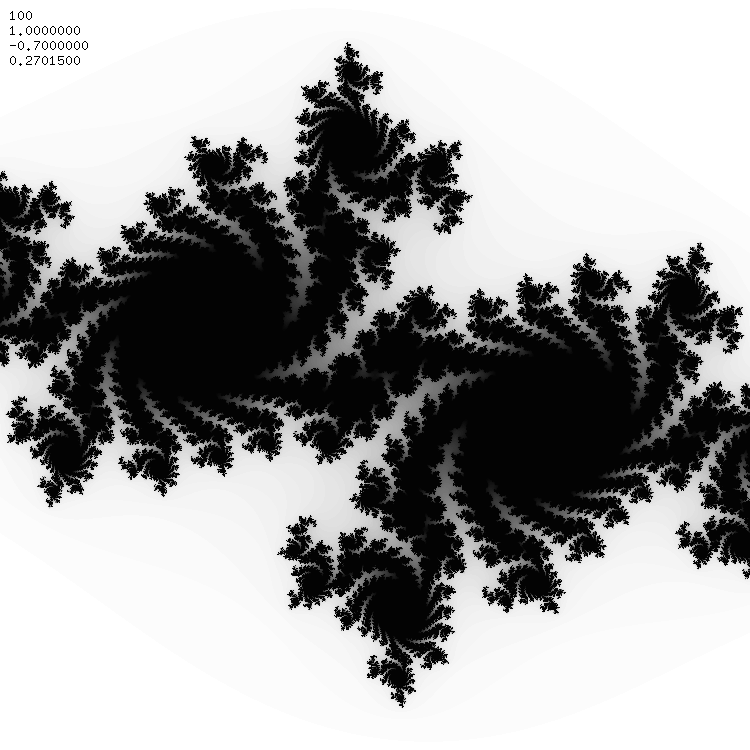
\includegraphics[width=0.2\textwidth]{images/Julia-Fractal.png}
  \caption{Exampelimage}
\end{figure}

\subparagraph{Unforgeability}
\label{subp:subparagraph_name}

Graphic by \url{http://en.wikipedia.org/wiki/Pretty_Good_Privacy#/media/File:PGP_diagram.svg}
